\documentclass[main.tex]{subfiles}

\begin{document}

% \textcolor{red}{Вводная лекция}

\section{Лекция 09.03.2021 (Донцов Е.В.)}

\subsection{Математическая модель полубесконечной трещины ГРП. Продолжение}

\includegraphics[width=\textwidth, page=30]{HF_slides_2021.pdf}

Я доработал вывод уравнений для модели полубесконечной трещины, поэтому давайте ещё раз его вспомним.
\\

Трудно сразу провести анализ полученной нами системы уравнений для модели плоской трещины.
Поэтому (чтобы понять происходящее) рассмотрим более простую задачу о полубесконечной трещине.
Это самая простая геометрия и для неё легче всего найти решение.

Что такое полубесконечная трещина?
Зачем она нужна?

Если рассмотрим задачу о плоской трещине и приблизимся к кончику трещины (т.е. мы хотим понять, что происходит возле границы трещины, когда она распространяется), то как раз получим геометрию полубесконечной трещины.
Понятно, что ничего полубесконечного в жизни не бывает, это некая математическая идеология, но необходимо понимать, что физически мы рассматриваем проблему возле кончика трещины.

Основные (изначальные) уравнения соответствуют плоской трещине.
Далее, чтобы перейти к полубесконечной трещине, мы рассматриваем проблему, в которой рассматриваемая трещина едет (распространяется) с некой постоянной скоростью $V$.

Вводим движущуюся систему координат (начало координат находится в кончике трещины, ось $O\hat{x}$ направлена внутрь трещины):
\beq
\hat{x}=Vt-x
\eeq

Предполагаем, что в этой системе координат задача стационарная, т.е. вся зависимость от времени зашита в $\hat{x}$ (нет ещё отдельной дополнительной зависимости от времени).

Тогда уравнение
\beq
\frac{\partial w}{\partial t}+\frac{\partial q}{\partial x}+\frac{C'}{\sqrt{t-t_0(x)}}=Q_{0,ps}(t)\delta(x)
\eeq
перепишется в виде обыкновенного дифференциального уравнения:
\beq
V\frac{dw}{d\hat{x}}-\frac{dq}{d\hat{x}}+\frac{C'}{\sqrt{\hat{x}/V}}=0
\eeq

Далее интегрируем полученное уравнение по $\hat{x}$:
\beq
\frac{w^2}{\mu'}\frac{dp}{d\hat{x}}=V+2C'\frac{\sqrt{V\hat{x}}}{w}
\eeq
(здесь учли, что $q=-\dfrac{w^3}{\mu'}\dfrac{\partial p}{\partial x}$).

Далее следующий шаг упрощения задачи: вместо прямого уравнения упругости используем обратное уравнение упругости, в котором открытие будет функцией градиента давления.
Самое главное, что в этой формулировке мы автоматически удовлетворяем критерию распространения.
Открытие будет равно некой корневой зависимости (т.е. это и есть критерий распространения) плюс некое слагаемое, зависящее от градиента давления.

Если интересно: все эти функции считаются через преобразование Фурье.
В Фурье-образах интегральное уравнение превращается в очень простое соотношение между давлением и открытием.

Итог: у нас было 4 уравнения (закон сохранения объёма, связь потока с градиентом давления, упругость и критерий распространения); после всех математических манипуляций остались только 2 уравнения.

\includegraphics[width=\textwidth, page=31]{HF_slides_2021.pdf}

Далее рассмотрим некий математический трюк, с помощью которого из оставшихся двух уравнений сделаем только одно уравнение.

Получили одно интегральное уравнение на открытие, в котором присутствуют все входные параметры задачи.

Далее производим масштабирование (обезразмеривание), т.е. вводим безразмерные переменные.
Идея в том, что после того, как мы отмасштабируем уравнение, мы получим очень простое безразмерное уравнение в представленной на слайде форме.

Фактически получили уравнение на одно безразмерное открытие $\tilde{w}$.

Важно то, что в полученном уравнении нет сингулярностей.

\includegraphics[width=\textwidth, page=32]{HF_slides_2021.pdf}

Итак, мы пришли к одному уравнению на безразмерное открытие, в котором есть 3 характерных слагаемых: первое (внеинтегральное) слагаемое описывает эффект трещиностойкости, второе слагаемое включает в себя эффект вязкости, третье слагаемое отвечает за утечки.

Соответственно выделяют 3 аналитических решения:

1) в случае доминирования трещиностойкости (при очень маленьких вязкости и утечках, например, закачиваем воду в практически непроницаемый резервуар);

2) в случае доминирования вязкости (чтобы трещиностойкость была пренебрежимо малой, можно представить себе, что мы закачиваем жидкость в уже существующую трещину) -- получается некое интегральное уравнение -- на следующем слайде будет представлено полное решение этого уравнения;

3) в случае доминирования утечек.

\includegraphics[width=\textwidth, page=33]{HF_slides_2021.pdf}

Теперь покажу вывод решения в случае доминирования вязкости.

Предполагаем решение в форме степенной функции, подставляем и находим константы (интеграл считается аналитически).

\includegraphics[width=\textwidth, page=34]{HF_slides_2021.pdf}

Теперь посмотрим, как выглядит полное решение.
Можем его найти численно.

На центральном графике на слайде: чёрная линия -- численное решение рассматриваемого интегрального уравнения (при некотором наборе входных параметров), цветными линиями показаны предельные аналитические решения.

Видим, что по порядку величины не ошибёмся, если возьмём максимум известных аналитических решений.

\includegraphics[width=\textwidth, page=23]{HF_slides_2022.pdf}

Даже в приближении решения в виде максимума предельных решений будет относительно неплохой ответ.

\includegraphics[width=\textwidth, page=36]{HF_slides_2021.pdf}

\includegraphics[width=\textwidth, page=37]{HF_slides_2021.pdf}

\subsection{Математическая модель плоской трещины ГРП. Продолжение}

\includegraphics[width=\textwidth, page=38]{HF_slides_2021.pdf}

\includegraphics[width=\textwidth, page=39]{HF_slides_2021.pdf}

\includegraphics[width=\textwidth, page=40]{HF_slides_2021.pdf}

\includegraphics[width=\textwidth, page=41]{HF_slides_2021.pdf}

\includegraphics[width=\textwidth, page=42]{HF_slides_2021.pdf}

\includegraphics[width=\textwidth, page=43]{HF_slides_2021.pdf}

\includegraphics[width=\textwidth, page=44]{HF_slides_2021.pdf}

\includegraphics[width=\textwidth, page=45]{HF_slides_2021.pdf}

\includegraphics[width=\textwidth, page=46]{HF_slides_2021.pdf}

\includegraphics[width=\textwidth, page=47]{HF_slides_2021.pdf}

\includegraphics[width=\textwidth, page=48]{HF_slides_2021.pdf}



\end{document}